
\title{Лекция 1\\Основные положения семантической технологии проектирования интеллектуальных компьютерных систем нового поколения \vspace{-2em}} 
\author[]{Шункевич Д.В.}
\institute[]{Белорусский государственный университет информатики и радиоэлектроники}

\begin{frame}
	\titlepage
\end{frame}

\begin{frame}{\\Содержание лекции}
	\vspace{10mm}
	\topline
	\justifying
	\begin{itemize}
		\item Понятие интеллекта, интеллектуальной системы, комплексной задачи.
		\item Основные положения семантической технологии проектирования интеллектуальных компьютерных систем нового поколения.
		\item Основные компоненты указанной технологии.
		\item Понятие информационной конструкции, формального языка, знака, синтаксиса, семантики.
		\item Понятие семантической памяти.
	\end{itemize}

\end{frame}

\begin{frame}{\\Интеллектуальная система}
	\vspace{10mm}
	\begin{SCn}
		\scnheader{Интеллектуальная система} 
		\scnidtf{система, которая может легко \underline{научиться решать} новые задачи} 
	\end{SCn}	
	\begin{scnrelfromset}{важно отличать}
		\scnitem {способность обучаться более качественному решению задач определенного ограниченного класса (как это делают классические нейросетевые модели)}
		\scnitem {способность относительно легко переходить от решения задач одного класса к решению задач другого класса (с ограничениями или без них)}
	\end{scnrelfromset}
\end{frame}

\begin{frame}{\\Комплексная задача}
	\vspace{10mm}
	\begin{SCn}
		\scnheader{Комплексная задача}
		\scnidtf{задача, для решения которой необходимо использовать \underline{различные виды заний} и \underline{различные модели} решения задач.}
	\end{SCn}
	\begin{scnrelfrom}{примечание}
	 	{Для комплексных задач невозможно заранее сказать, какой набор моделей потребуется для решения}
	\end{scnrelfrom}
	\vspace{5mm}
	Примеры комплексных задач:
	\begin{itemize}
		\item понимание естественных языков, изображений, речевых сообщений 
		\item планирование поведения интеллектуальных роботов.
	\end{itemize}
\end{frame}

\begin{frame}{\\Гибридная интеллектуальная система}
	\vspace{10mm}
	\begin{SCn}
	\scnheader{Гибридная интеллектуальная система} \scnidtf{интеллектуальная система, интегрирующая различные виды знаний и различные модели решения задач}
	\end{SCn}
	\begin{scnrelfrom}{примечание}
		{Именно ГИС способны решать комплексные задачи}
	\end{scnrelfrom}
	\begin{scnrelfromset}{недостатки}
		\scnitem{монолитность}
		\scnitem{решение конкретной задачи, а не различных классов задач}
		\scnitem{разработка требует колоссальных ресурсов}
		\scnitem{практически невозможно повторно использовать какие-либо компоненты систем для решения других задач, необходимо все делать заново}
	\end{scnrelfromset}
\end{frame}

\begin{frame}{\\OSTIS}
	\vspace{10mm}
	\begin{SCn}
	\scnheader{OSTIS}
	\scnidtf{Open Semantic Technology for Intelligent Systems}
	\scnidtf{открытая комплексная технология проектирования совместимых интеллектуальных систем.}
	\vspace{3mm}
	Основные положения:
		\begin{itemize}
		\item база знаний OSTIS может описывать любой вид знаний
		\item решатель задач OSTIS основан на многоагентном подходе и позволяет легко комбинировать любые модели решения задач
		\item интерфейс ostis-системы представляет собой подсистему со своей БЗ и решателем задач (также может быть описан с помощью SC-кода)
		\item использование универсального способа представления (кодирования) информации, получившего название SC-код 
	\end{itemize}
	\end{SCn}
\end{frame}

\begin{frame}{\\Достоинства OSTIS}	
	\vspace{5mm}
	\begin{itemize}
		\item Унифицированность (единообразие) представления (любая информация может быть представлена одним и тем же способом)
		\item Удобство машинной обработки и восприятия человеком
		\item Любые знания и модели решения задач могут быть легко интегрированы в ostis-систему (по принципу plug \& play). Систему всегда можно переобучить для решения другой задачи
		\item Компоненты ostis-систем универсальны и совместимы друг с другом. Можно создавать библиотеку компонентов и использовать их повторно (что позволяет сократить время разработки новых компонентов на 40-60\%)
		\item Система описывается с помощью SC-кода, поэтому она может анализировать себя, искать в себе ошибки и оптимизировать собственную работу, то есть обладает рефлексивностью
	\end{itemize}
\end{frame}

\begin{frame}{\\Достоинства OSTIS}
	\vspace{10mm}
	\begin{itemize}
		\item Платформенная независимость. Разработка ostis-системы осуществляется независимо от операционной системы и архитектуры компьютера. Платформа может быть реализована как в программном варианте (виртуальная машина), так и в аппаратном варианте
		\item Благодаря особому многоагентному подходу ostis-системы ориентированы на параллельную обработку информации
		\item Ostis-система может включать в себя компоненты, разработанные на базе OSTIS, а также объединяться с любыми другими системами и интегрировать другие компоненты через специальный протокол обмена информацией (JSON) и/или программный интерфейс (API)
		\item Производительность ostis-системы не хуже традиционной системы, а в иногда может оказаться лучше за счет параллельной обработки. При переходе на семантические компьютеры производительность будет еще выше.
	\end{itemize}
\end{frame}
  
\begin{frame}{\\Важно понимать}
	\vspace{10mm}
	\begin{itemize}
		\item  OSTIS -- это не конкретная интеллектуальная система, а технология разработки интеллектуальных систем, каждая из которых, в свою очередь, будет решать задачи определенного класса
		\item Ключевые преимущества OSTIS заключаются не в принципиально новых функциональных возможностях разрабатываемых систем (большинство функций ostis-систем можно реализовать с помощью традиционных средств), а в том, насколько легко модифицировать и развивать разрабатываемые системы, адаптировать их к новым задачам, а также насколько эффективно можно накапливать и использовать полученные компоненты при разработке новых систем, сокращая при этом время и трудоемкость их разработки
		\item OSTIS -- это способ решения проблемы совместимости, одной из важнейших проблем современных технологий
	\end{itemize}
\end{frame}	

\begin{frame}{\\Архитектура ostis-системы}
	\vspace{10mm}
	\begin{center} 
		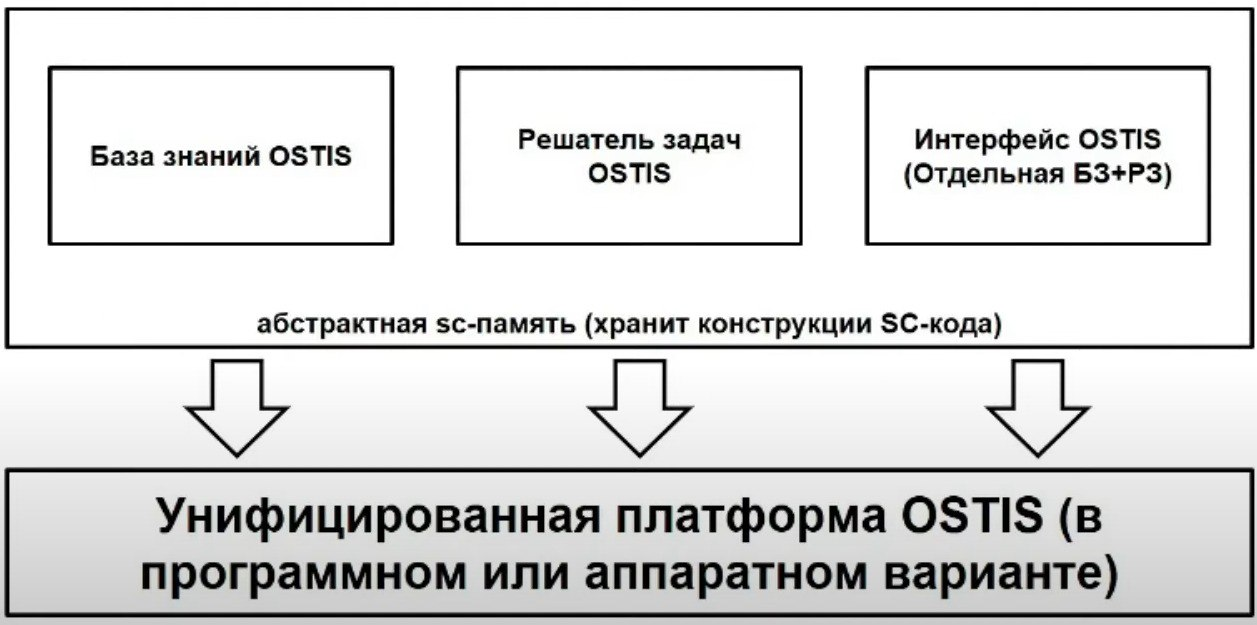
\includegraphics[width=120mm]{./part1/pictures/scheme.jpeg}
	\end{center}
\end{frame}

\begin{frame}{\\Архитектура ostis-системы}
	\vspace{10mm}
	\begin{itemize}
		\item База знаний OSTIS может описывать любой вид знаний, при этом её легко дополнять новыми видами знаний.
		\item Решатель задач OSTIS основан на многоагентном подходе и позволяет легко интегрировать и комбинировать любые модели решения задач.
		\item Интерфейс  ostis-системы представляет собой подсистему со своей базой знаний и решателем задач, т.е. так же может быть описан с помощью SC-кода.
	\end{itemize}
	
\end{frame}

\begin{frame}{\\Понятие семантической памяти}
	
\end{frame}

\begin{frame}{\\Информационная конструкция}
	\vspace{10mm}
	\begin{SCn}
	\scnheader{Информационная конструкция}
	\scnidtf{конструкция (структура), содержащая некоторые сведения о некоторых сущностях}	
	\vspace{5mm}
	Информационная конструкция -- множество, на котором задано
		\begin{itemize}
			\item Отношение \underline{синтаксической} эквивалентности и семейство классов синтаксической эквивалентности информационных конструкций
			\item Отношение \underline{семантической} эквивалентности и семейство классов семантической эквивалентности информационных конструкций 
			\item Отношение \underline{логической} эквивалентности и семейство классов логической эквивалентности информационных конструкций.
		\end{itemize} 
	\end{SCn}
\end{frame}

\begin{frame}{\\Формальный язык}
	\begin{SCn}
		\scnheader{язык}  
		\scnidtf{множество информационных конструкций, построенных по общим синтаксическим и семантическим правилам}
		
		\scnheader{формальный язык}  
		\scnidtf{язык, в котором значение каждого слова или знака, правила построения предложений и понимания их смысла однозначны.}
		\scnidtf{множество строк над конечным алфавитом языка}		
	\end{SCn}
\end{frame}

\begin{frame}{\\Знак}
	\begin{SCn}
		\scnheader{знак}
		\scnidtf{фрагмент информационной конструкции, обладающий свойством, \underline{обозначать} некоторую сущность (объект), которая наряду с другими сущностями описывается указанной информационной конструкцией}
	%	\begin{scnrelfromset}{пояснение}
	%		\scnitem {Hello}
	%	\end{scnrelfromset}
	\end{SCn}
\end{frame}

\begin{frame}{\\Синтакис и семантика}
	\scnheader{синтаксис}
	\scnidtf{наука, изучающая отношения между знаками}
	\scnheader{семантика}
	\scnidtf{наука, изучающая отношения между знаками и их значениями}
\end{frame}





